\documentclass[english,hidelinks,pdftex, 11 pt, class=report,crop=false]{standalone}
\usepackage[T1]{fontenc}
\usepackage[utf8]{luainputenc}
\usepackage{lmodern} % load a font with all the characters
\usepackage{geometry}
\geometry{verbose,a4paper, inner=0cm, outer=0 cm, bmargin=2cm, tmargin=1cm}
%\textwidth=12cm
\setlength{\parindent}{0bp}
\usepackage{import}
\usepackage[subpreambles=false]{standalone}
\usepackage{amsmath}
\usepackage{amssymb}
\usepackage{esint}
\usepackage{babel}
\usepackage{tabu}
\usepackage[dvipsnames, table]{xcolor}
\usepackage{cancel}
\makeatother
\makeatletter
\usepackage{datetime2}
\usepackage{titlesec}
\usepackage[many]{tcolorbox}

% Eheter
\newcommand{\enh}[1]{\,\textrm{#1}}
%referances
\newcommand{\net}[2]{{\color{blue}\href{#1}{#2}}}

%Spaces
\newcommand{\vsk}{\\[12pt]}
\newcommand{\vs}{\vspace{-12pt}}

% Tabell for opplegg

\newcommand{\ovlist}[1]{
\vspace{-16pt}
\begin{itemize}
	#1
\end{itemize}
}

% Chapters and sections
\titleformat{\section}[block]{\bfseries}{\hspace{3cm}\thesection}{5pt}{}
\titleformat{\subsection}[block]{\bfseries}{\hspace{3cm}\thesection}{5pt}{}
\newcommand{\sectionbreak}{\clearpage} % New page on each section
 

\newlength{\mywidth}
\setlength{\mywidth}{14cm}

\newcommand{\cont}[1]{
\begin{tcolorbox}[center, boxrule=0.0 mm, width=\mywidth,arc=0mm,enhanced jigsaw,,colback=white,breakable]
#1	
\end{tcolorbox}
}

\newcommand{\info}[5]{
\begin{tcolorbox}[center, boxrule=0.1 mm, width=\mywidth,arc=0mm,enhanced jigsaw,breakable,colback=yellow!5]	
	
	\footnotesize
	\textbf{Øvingsområde}\\[5pt] #1 
	
	\textbf{Utstyr}\\ #2  \\
	
	\begin{tabular}{@{} p{4cm} p{4cm} l} 
		\textbf{Tid} & \textbf{Elevinndeling} & \textbf{Læringsarena} \\
		#3  & #4 & #5
	\end{tabular} 
\end{tcolorbox}	
}

\newcommand{\gjen}[1]{\begin{tcolorbox}[center,boxrule=0.1 mm, width=\mywidth,arc=0mm,colback=blue!3] {\large \textbf{Gjennomføring} \vspace{5 pt}}\newline #1  \end{tcolorbox}\vspace{-5pt}}
\newcommand{\eks}[1]{\begin{tcolorbox}[center,boxrule=0.1 mm, width=\mywidth,arc=0mm,colback=green!3] {\large \textbf{Eksempel} \vspace{5 pt}}\newline #1  \end{tcolorbox}\vspace{-5pt}}

\newcounter{opl}
%\numberwithin{opl}{article}


\newcommand{\opl}[1]{
\newpage
{\refstepcounter{opl} %\phantomsection 
\large \textbf{\theopl \;#1} \vsk}
}

% Headlines
\newcommand{\fork}{\textbf{Forkunnskapar}\\}
\newcommand{\forb}{\textbf{Forberedelsar}\\}
\newcommand{\opgvr}{\textbf{Oppgaver}}



%colors
\newcommand{\colr}[1]{{\color{red} #1}}
\newcommand{\colb}[1]{{\color{blue} #1}}
\newcommand{\colo}[1]{{\color{orange} #1}}
\newcommand{\colc}[1]{{\color{cyan} #1}}
\definecolor{projectgreen}{cmyk}{100,0,100,0}
\newcommand{\colg}[1]{{\color{projectgreen} #1}}

% Lister med bokstavar
\usepackage[inline]{enumitem}
% Opg
\newcommand{\abc}[1]{
	\begin{enumerate}[label=\alph*),leftmargin=18pt]
		#1
	\end{enumerate}
}

\usepackage[]{hyperref}

\newcommand{\note}{Merk}
\newcommand{\notesm}[1]{{\footnotesize \textsl{\note:} #1}}
\newcommand{\ekstitle}{Eksempel }
\newcommand{\sprtitle}{Språkboksen}
\newcommand{\expl}{forklaring}
\newcommand{\pyt}{Pytagoras' setning}
\newcommand\sv{\vsk \textbf{Svar} \vspace{4 pt}\\}

%references
\newcommand{\reftab}[1]{\hrs{#1}{tabell}}
\newcommand{\rref}[1]{\hrs{#1}{regel}}
\newcommand{\dref}[1]{\hrs{#1}{definisjon}}
\newcommand{\refkap}[1]{\hrs{#1}{kapittel}}
\newcommand{\refsec}[1]{\hrs{#1}{seksjon}}
\newcommand{\refdsec}[1]{\hrs{#1}{delseksjon}}
\newcommand{\refved}[1]{\hrs{#1}{vedlegg}}
\newcommand{\eksref}[1]{\textsl{#1}}
\newcommand\fref[2][]{\hyperref[#2]{\textsl{figur \ref*{#2}#1}}}
\newcommand{\refop}[1]{{\color{blue}Oppgave \ref{#1}}}
\newcommand{\refops}[1]{{\color{blue}oppgave \ref{#1}}}


%Algebra
\newcommand{\kvadset}{Kvadratsetningene}
\newcommand{\aenato}{Sum-produkt-metoden}

% Geometry
\newcommand{\hlikb}{Midtnormalen i en likebeint trekant}
\newcommand{\arealsetn}{Arealsetningen}
\newcommand{\trkmedian}{Median}
\newcommand{\midtrk}{Midtnormal (i trekant)}
\newcommand{\innskrsirk}{Innskrevet sirkel}
\newcommand{\cossetn}{Cosinussetningen}
\newcommand{\perfvink}{Sentral- og periferivinkel}
\newcommand{\tang}{Tangent}

% Derivative
\newcommand{\derel}{Den deriverte av elementære funksjoner}
\newcommand{\divder}{Divisjonsregelen}
\newcommand{\kjernereg}{Kjerneregelen}
\newcommand{\prodregder}{Produktregelen}
\newcommand{\lhop}{L'Hopitals regel}

% Funksjonsdrofting
\newcommand{\monder}{Monotoniegenskaper og den deriverte}
\newcommand{\fderekstr}{$ \bm{f'=0} $ for lokale ektstremalpunkt}
\newcommand{\andredertest}{Andrederiverttesten}

% Vectors
\newcommand{\detar}{Arealformler med determinanter}
\newcommand{\avstpunktlin}{Avstand mellom punkt og linje}

%Appendix
\newcommand{\rolle}{Rolles teorem}
\newcommand{\meanval}{Middelverdisetningen}

% Solutions manual
\newcommand{\selos}{Se løsningsforslag.}

\begin{document}
\subsection*{Kapittel \ref{Trigonometri}}	
\footnotesize
For alle svar tas det for gitt at $ n\in \mathbb{Z} $.

\textsl{Merk}: Uttrykkene for løsninger av trigonometriske ligninger kan se forskjellige ut, men gi de samme verdiene av $ x $. For eksempel vil $ {x= 2\pi n-\frac{\pi}{4}} $ være den samme løsningen som $ {x = \frac{7\pi}{4}+2\pi n} $ fordi $ {-\frac{\pi}{4}+2\pi = \frac{7\pi}{4}}$. Vi kan alltid trekke ut heltallsfaktorer av $ n $-leddet for å endre på uttrykk, for å sjekke om ditt svar er riktig bør du derfor først sjekke at ditt $ n $-ledd er i overensstemmelse med fasit.

\opr{udir}
Siden radiusen til enhetssirkelen er $ 1 $, blir forholdet mellom buelengde $ l $ og radiusen lik $ \frac{l}{1}=l $.

\opr{rads} \textbf{a)} $ \frac{\pi}{3} $ \textbf{b)} $ \frac{\pi}{12} $

\opr{grad} \textbf{a)} $ 165^\circ $ \textbf{b)} $ 330^\circ $

\opr{pytg} Se løsningsforslag.

\opr{tanx} \textbf{a)} $ 0  $ \textbf{b)} $- \frac{1}{\sqrt{3}} $
\newpage
\opr{kvadrant}\\
\begin{tabular}{@{}l|c| c| c|c|}
	
	&1. kvadrant & 2. kvadrant & 3. kvadrant & 4. kvadrant\\ \hline
	$ \sin x $& +& +& $ - $&$ - $\\ \hline
	$ \cos x $& +& $ - $& $ - $&+\\ \hline
	$ \tan x $& +& $ - $& +&$ - $\\\hline
\end{tabular}\vsk

\opr{trigverd}
\textbf{a)} $ -\frac{1}{2} $ \textbf{b)} $ -1 $ \textbf{c)} $ 0 $ \textbf{d)} $ -\sqrt{3} $

\opr{averdier} 
\textbf{a)} 0 \textbf{b)} $ \frac{\pi}{3} $ \textbf{c)} $ \pi $
\textbf{d)} $ \frac{3\pi}{4} $ \textbf{e)} $ \frac{\pi}{4} $ 
\textbf{f)} $ \frac{\pi}{6} $

\opr{bruk1} \selos

\opr{sin2xopg} \textbf{a)} Se side \pageref{sin2xbevis}. \textbf{b)} Se løsningsforslag.

\opr{cossomsin} $ \sin(3x) $

\opr{cossinsin} \textbf{a)} $2\sin\left(2x+\frac{2\pi}{3}\right)  $ 

\opr{sincos0} Se løsningsforslag.

\opr{triligns} \textbf{a)} $ x = \pm \frac{\pi}{4}+2\pi n $ \textbf{b)} $ x=\frac{3}{2} \vee x = \frac{9}{2} $ \textbf{c)} $ x=\frac{1}{3}(\frac{\pi}{6}+2\pi n)\vee x= \frac{1}{3}(\frac{5\pi}{6}+2\pi n) $ \textbf{d)} $ x=\frac{\pi}{3}(3n+1)\vee x= \frac{\pi}{6}(6 n+1)$ \textbf{e)} $\frac{1}{4}(\pi n-\frac{\pi}{3} )$

\opr{asinbcos0o} \textbf{a)} $ \frac{\pi}{6}+\pi n $ \textbf{b)} $ \pi n-\frac{\pi}{3} $ \textbf{c)} $ \frac{1}{2}\left(\pi n-\frac{\pi}{4}\right) $

\opr{kombo}
\textbf{a)} $ x=2\pi n-\frac{\pi}{4} $
\textbf{b)} $ x\pi^2(4n-1)\vee x=2\pi\left(\frac{\pi}{6}+2\pi n\right) $ 

\opr{abctri}
\textbf{a)} ${ x= 2\pi n-\frac{\pi}{2} \vee x = \frac{\pi}{6}+2\pi n \vee x = \frac{5\pi}{6}+2\pi n}$ \textbf{b)} ${ x=\frac{1}{3}(\pi +2\pi n) }$ \textbf{c)} ${ x = \pm \frac{3\pi}{4}+2\pi n  }$ \textbf{d)} ${ x=\frac{1}{3}+n }$ \textbf{e)} ${ x=\frac{1}{3}(\pi +2\pi n) }$

\opr{kvadopg}
\textbf{a)} a) $ x = \pm \frac{\pi}{6}+\pi n $ \textbf{b)} $ \pm \pi + 4\pi n$ (eventuelt $ x=\pi +2\pi n) $)

\opr{cosmaks} Se løsningsforslag.

\opr{cosfunko} \textbf{a)} $ P = \frac{2\pi}{3} $ \textbf{b)} $ f_{maks}=9 $, $ f_{min}=-1 $ \textbf{c)} $ f $ har maksimum for $ x= \frac{1}{3}\left(2\pi n-\frac{\pi}{12}\right) $ og minimum for $ x=\frac{1}{3}(2\pi n-\frac{11\pi}{12}) $

\opr{sinfnpkt} \textbf{a)} $ P=4 $ \textbf{b)} $ (-1, 3) $ og $ (3, 3) $ \textbf{c)}  $ x=-\frac{7}{3} $, $ x=\frac{5}{3} $ og $ x=\frac{1}{3} $

\opr{skissin}\\
\vs
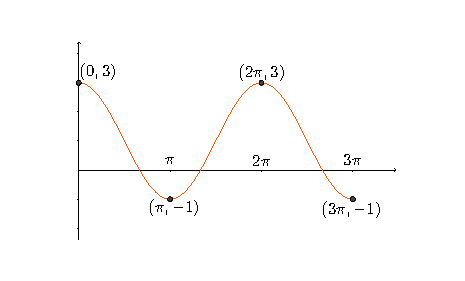
\includegraphics[]{skissin}\vs

\opr{sincosfig}
\textbf{a)} $ 3\cos(\pi x - \pi) +2 $ \textbf{b)} $ 3\sin\left(\pi x-\frac{\pi}{2}\right) +2 $

\grubr{opgtangr}


\end{document}

